% rmep_arch_schematic.tex
% Compile: pdflatex rmep_arch_schematic.tex
\documentclass[border=8pt,tikz]{standalone}
\usepackage{tikz}
\usetikzlibrary{positioning,arrows.meta,fit,backgrounds,calc}

\begin{document}
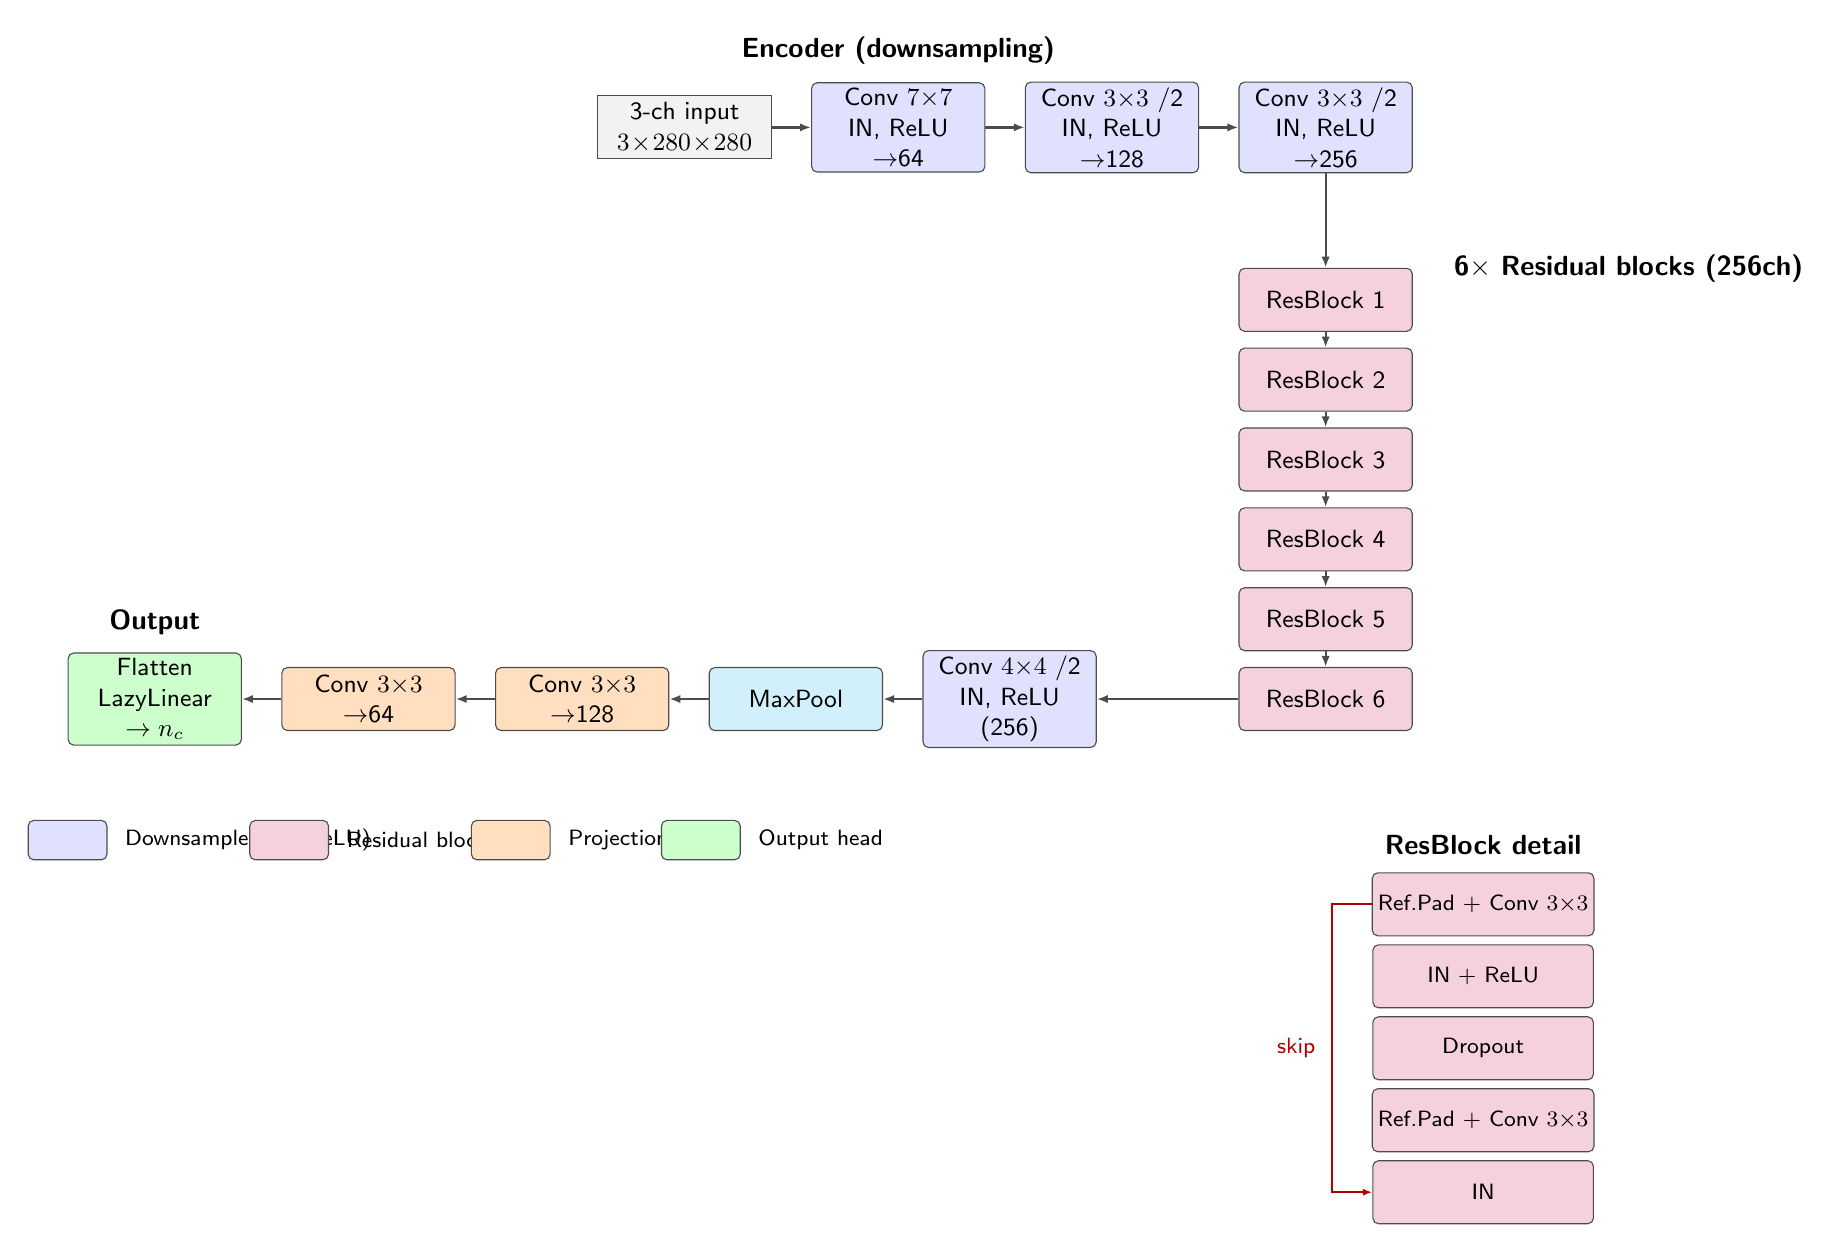
\begin{tikzpicture}[
  font=\sffamily\small,
  every node/.style={align=center},
  inp/.style ={rectangle, draw=black!70, fill=gray!10,
               minimum width=22mm, minimum height=8mm, inner sep=2pt},
  ds/.style  ={rectangle, rounded corners=2pt, draw=black!70, fill=blue!12,
               minimum width=22mm, minimum height=9mm, inner sep=2pt},
  res/.style ={rectangle, rounded corners=2pt, draw=black!70, fill=purple!18,
               minimum width=22mm, minimum height=8mm, inner sep=2pt},
  proj/.style={rectangle, rounded corners=2pt, draw=black!70, fill=orange!25,
               minimum width=22mm, minimum height=8mm, inner sep=2pt},
  pool/.style={rectangle, rounded corners=2pt, draw=black!70, fill=cyan!18,
               minimum width=22mm, minimum height=8mm, inner sep=2pt},
  head/.style={rectangle, rounded corners=2pt, draw=black!70, fill=green!20,
               minimum width=22mm, minimum height=9mm, inner sep=2pt},
  arrow/.style={-{Latex[length=1.4mm]}, thick, draw=black!70},
]

% Linear left->right pipeline
\node[inp]                    (in)   {3-ch input\\$3\!\times\!280\!\times\!280$};
\node[ds,   right=5mm of in]  (ds1)  {Conv $7{\times}7$\\IN, ReLU\\$\to$64};
\node[ds,   right=5mm of ds1] (ds2)  {Conv $3{\times}3$ /2\\IN, ReLU\\$\to$128};
\node[ds,   right=5mm of ds2] (ds3)  {Conv $3{\times}3$ /2\\IN, ReLU\\$\to$256};

% Stack of 6 residual blocks
\node[res,  below=12mm of ds3] (r1) {ResBlock 1};
\node[res,  below=2mm  of r1]  (r2) {ResBlock 2};
\node[res,  below=2mm  of r2]  (r3) {ResBlock 3};
\node[res,  below=2mm  of r3]  (r4) {ResBlock 4};
\node[res,  below=2mm  of r4]  (r5) {ResBlock 5};
\node[res,  below=2mm  of r5]  (r6) {ResBlock 6};

% Continue pipeline below
\node[ds,   left=14mm of r6, xshift=-4mm] (ds4) {Conv $4{\times}4$ /2\\IN, ReLU\\(256)};
\node[pool, left=5mm of ds4]              (mp)  {MaxPool};
\node[proj, left=5mm of mp]               (p1)  {Conv $3{\times}3$\\$\to$128};
\node[proj, left=5mm of p1]               (p2)  {Conv $3{\times}3$\\$\to$64};
\node[head, left=5mm of p2]               (fc)  {Flatten\\LazyLinear\\$\to n_c$};

% Arrows top row
\draw[arrow] (in)  -- (ds1);
\draw[arrow] (ds1) -- (ds2);
\draw[arrow] (ds2) -- (ds3);

% ds3 -> residual stack
\draw[arrow] (ds3.south) -- (r1.north);
\draw[arrow] (r1) -- (r2);
\draw[arrow] (r2) -- (r3);
\draw[arrow] (r3) -- (r4);
\draw[arrow] (r4) -- (r5);
\draw[arrow] (r5) -- (r6);

% r6 -> ds4 (transition to lower row, going right-to-left)
\draw[arrow] (r6) -- (ds4);
\draw[arrow] (ds4) -- (mp);
\draw[arrow] (mp)  -- (p1);
\draw[arrow] (p1)  -- (p2);
\draw[arrow] (p2)  -- (fc);

% -------- labels ----------------------------------------------------------
\node[above=1mm of ds1, font=\sffamily\bfseries] {Encoder (downsampling)};
\node[above=1mm of r1.east, anchor=south west, xshift=4mm, font=\sffamily\bfseries]
     {6$\times$ Residual blocks (256ch)};
\node[above=1mm of fc, font=\sffamily\bfseries] {Output};

% Residual-block detail box
\begin{scope}[shift={($(r6.south)+(20mm,-22mm)$)}, font=\sffamily\footnotesize]
  \node[res, minimum width=28mm] (rd0) {Ref.Pad + Conv $3{\times}3$};
  \node[res, minimum width=28mm, below=1mm of rd0] (rd1) {IN + ReLU};
  \node[res, minimum width=28mm, below=1mm of rd1] (rd2) {Dropout};
  \node[res, minimum width=28mm, below=1mm of rd2] (rd3) {Ref.Pad + Conv $3{\times}3$};
  \node[res, minimum width=28mm, below=1mm of rd3] (rd4) {IN};
  \node[font=\sffamily\bfseries, above=1mm of rd0] {ResBlock detail};
  % residual connection arrow
  \draw[-{Latex[length=1.2mm]},thick,red!70!black]
        (rd0.west) -- ++(-5mm,0) |- (rd4.west);
  \node[red!70!black, left=6mm of rd2, font=\sffamily\footnotesize] {skip};
\end{scope}

% -------- legend ----------------------------------------------------------
\begin{scope}[shift={($(fc.south west)+(0,-12mm)$)}, font=\sffamily\footnotesize]
  \node[ds,   minimum width=10mm, minimum height=5mm] (lg1) {};
  \node[right=1mm of lg1] {Downsample (IN+ReLU)};
  \node[res,  minimum width=10mm, minimum height=5mm, right=18mm of lg1] (lg2) {};
  \node[right=1mm of lg2] {Residual block};
  \node[proj, minimum width=10mm, minimum height=5mm, right=18mm of lg2] (lg3) {};
  \node[right=1mm of lg3] {Projection};
  \node[head, minimum width=10mm, minimum height=5mm, right=14mm of lg3] (lg4) {};
  \node[right=1mm of lg4] {Output head};
\end{scope}

\end{tikzpicture}
\end{document}